\documentclass[conference]{IEEEtran}
\IEEEoverridecommandlockouts
% The preceding line is only needed to identify funding in the first footnote. If that is unneeded, please comment it out.

% RESEARCH QUESTION
% What attributes/charateristics in songs have the most dominant effect in playlist generation

\usepackage{tabularx,booktabs}
% defined centered version of "X" column type:
\newcolumntype{C}{>{\centering\arraybackslash}X} 

\usepackage{url}
\usepackage{listings}
\usepackage{color}

\usepackage{blindtext}
\usepackage{geometry}
 \geometry{
 a4paper,
 total={170mm,257mm},
 left=25mm,
 right=25mm,
 top=25mm,
 }

\usepackage{subfig}

\definecolor{dkgreen}{rgb}{0,0.6,0}
\definecolor{gray}{rgb}{0.5,0.5,0.5}
\definecolor{mauve}{rgb}{0.58,0,0.82}

\lstset{frame=tb,
  language=Python,
  aboveskip=3mm,
  belowskip=3mm,
  showstringspaces=false,
  columns=flexible,
  basicstyle={\small\ttfamily},
  numbers=none,
  numberstyle=\tiny\color{gray},
  keywordstyle=\color{blue},
  commentstyle=\color{dkgreen},
  stringstyle=\color{mauve},
  breaklines=true,
  breakatwhitespace=true,
  tabsize=3
}

\usepackage{cite}
\usepackage{amsmath,amssymb,amsfonts}
\usepackage{algorithmic}
\usepackage{graphicx}
\usepackage{textcomp}
\usepackage{xcolor}
\def\BibTeX{{\rm B\kern-.05em{\sc i\kern-.025em b}\kern-.08em
    T\kern-.1667em\lower.7ex\hbox{E}\kern-.125emX}}
\begin{document}

\title{Effects of Centrality on Network Topology in Music Playlists\\
{\footnotesize \textsuperscript{} Digital Media and Social Networks - Undergraduate Group 34}
}

\author{\IEEEauthorblockN{1\textsuperscript{st} Conrad Bennett}
\IEEEauthorblockA{\textit{Electronic Engineering and Computing Science} \\
\textit{Queen Mary University of London}}
\and
\IEEEauthorblockN{2\textsuperscript{nd} A. J. Catak}
\IEEEauthorblockA{\textit{Electronic Engineering and Computing Science} \\
\textit{Queen Mary University of London}}
\and
\IEEEauthorblockN{3\textsuperscript{rd} Lewis Can Charles}
\IEEEauthorblockA{\textit{Electronic Engineering and Computing Science} \\
\textit{Queen Mary University of London}}
\and
\IEEEauthorblockN{4\textsuperscript{th} James Davies}
\IEEEauthorblockA{\textit{Electronic Engineering and Computing Science} \\
\textit{Queen Mary University of London}}

}

\maketitle

\begin{abstract}
Music streaming services have actively been trying to solve one of the more challenging issues within music-based content in recent years, in which playlists are extended without user input other than the existing songs in the playlist (target songs). This is called Automatic Playlist Continuation (APC), and it is an active area of research, both due to outstanding questions within the field and the fact that it is a consumer driven issue. This paper outlines the effects that centrality can have on the topology of song to song co-occurrence in music playlists, and which attributes have the most potential to have an effect on APC.

\end{abstract}

\begin{IEEEkeywords}
music playlists, co-occurrence networks, centrality, network topology, automatic playlist continuation
\end{IEEEkeywords}

\section{Introduction}
Music streaming platforms such as Spotify have revolutionized the music industry by offering a vast and diverse library of music, in tandem with personalized recommendation algorithms, which suggests songs to the user that are similar based on the listeners preferences. Automatic Playlist Continuation [4], implemented as Smart Shuffle in Spotify, is a feature which seamlessly extends playlists by adding similar music to the queue; quickly becoming an increasingly important feature in curating and personalising playlists [7]. A desirable characteristic of algorithm-curated playlists is generally perceived to be homogeneity when it comes to style or genre [9]. However, the inner workings of the Smart Shuffle algorithms are not explicitly disclosed, so how exactly the system tailors the continued playlist to specific users music tastes remains a mystery. \\

In order to understand this algorithm, we need to analyse the characteristics behind the music. How are links between how songs of the same genre grouped? Can the ‘context’ of a playlist can be defined based on the genres alone? By asking these questions we can focus on how the algorithm infers patterns from these playlist-based networks to recommend music. Typical analysis of characteristics in this vein were done via implicit feedback/explicit ratings [11] in addition to collaborative filtering [5], the latter of which is a process where recommendation algorithms assess probability that a user will enjoy certain content based on existing data i.e., "users that liked this also bought this" [3]. The project aims to see how effective playlist continuation is through centrality measures, co-occurrences and genre-specific patterns; determining whether or not the system can function as specified based purely on a song’s attributes and characteristics. We will primarily investigate this through analysis with the visualization of networks given the data and cohesion between their links and nodes. 

\subsection{Problem Statement}

There are many existing problems with recommendation systems that mean that song-song relationships within playlists aren't accurately captured. These can include popularity bias [14], the cold-start problem [15] or the lack of understanding in regard to the 'context' of the playlist [8]. It is therefore necessary to explore methodologies in which we can gain a more thorough understanding of the playlist context, and semantic value of the song-song relationships within it. \\

\begin{table*}[hbt!]
\centering
\caption{Network Statistics - Small Dataset}
\label{table:kysymys}
\begin{tabularx}{\textwidth}{@{} l *{5}{C} c @{}}

        \toprule
        Metric & Max. & Min. & Average & Median \\
        \midrule
        Degree & 87 & 9 & 28.7337 & 26 \\
        Degree Centrality & 0.0168 & 0.0536 & 0.0599 & 0.0485 \\
        Closeness Centrality & 0.4250 & 0.2183 & 0.3101 & 0.3082 \\
        Betweenness Centrality & 0.1288 & 0.0 & 0.0004 & 0.0 \\
        Eigenvector Centrality & 0.1578 & 4.0842 & 0.0180 & 0.0032 \\
        Clustering Coefficient & 1.0 & 0.4120 & 0.9352 & 1.0 \\
        Path Length & n/a & n/a & 3.2991 & n/a \\
        \bottomrule
        
    \end{tabularx}
    
\end{table*}

\begin{table*}[hbt!]
\centering
\caption{Network Statistics - Large Dataset}
\label{table:kysymys}
\begin{tabularx}{\textwidth}{@{} l *{10}{C} c @{}}

        \toprule
        Metric & Max. & Min. & Average & Median \\
        \midrule
        Degree & 776 & 9 & 165.7998 & 139 \\
        Degree Centrality & 0.2805 & 0.0032 & 0.0599 & 0.0503 \\
        Closeness Centrality & 0.5785 & 0.3422 & 0.4677 & 0.4748 \\
        Betweenness Centrality & 0.0081 & 0.0 & 0.0004 & 0.0001 \\
        Eigenvector Centrality & 0.0773 & 8.1146 & 0.0142 & 0.0106 \\
        Clustering Coefficient & 1.0 & 0.1804 & 0.5820 & 0.5291 \\
        Path Length & n/a & n/a & 2.1579 & n/a \\
        \bottomrule
        
    \end{tabularx}

\end{table*}

\section{Related Work}

\subsection{Co-Occurrence Networks}

Co-occurrence networks are instrumental in visualizing the relationships between nodes, providing a bidirectional view of song connections within playlists. In these networks, an edge represents the mutual occurrence of two songs, reflecting their shared presence without implying a sequence. 

\subsection{Network Analyses}

We can investigate the structure of undirected networks, and the relationships between nodes to discern prevalent patterns within the wider network and the topology associated with these patterns. For instance, we can use the Clustering Coefficient of a network, which is the probability that two network neighbours of a node are also neighbours of each other. In the context of playlist-based networks, it is the probability that if A is similar to B \textit{and} C, then B and C are similar as well , indicating a similarity in their attributes or listener preferences [3]. 

\begin{equation}
\label{}
CG = \frac{1}{N}\sum_{i} C_{i}
\end{equation}

\subsection{Centrality Measures}

Centrality measures provide a methodology in which we can quantify the nature of a node in regards to it's importance/relationship within the wider network. There are pros and cons to each of these specific measures, with most centrality measures suffering from various types of noise [12]. \\

\subsubsection{Degree Centrality}

The degree centrality can be defined as the number of edges attached to a node [12]. This measure can be used as a metric for the influence of a specific artist, genre, or song when it comes to analysis of playlist based data [2].

\begin{equation}
\label{}
c_i^{(degree)} = \sum_{j=1}^{N}A_{ij}
\end{equation}

\subsubsection{Closeness Centrality}

The closeness centrality is defined via the length between two nodes, i and j [12].

\begin{equation}
\label{}
c_i^{(closeness)} = \frac{N}{\sum_{j=1, j \neq i}^{N}d_{ij}}
\end{equation}

\subsubsection{Betweenness Centrality}

Betweeness centrality is based on closeness centrality, and revolves around the number of shortest paths from a to b, comparative to the number of those shortest paths specified that pass through another node [12].

\begin{equation}
\label{}
c_i^{(betweenness)} = \sum_{a \neq i \neq b}  \frac{\sigma_{ab}(i)}{\sigma_{ab}}
\end{equation}

\subsubsection{Eigenvector Centrality}

Eigenvector centrality extends the analysis of specific nodes to it's surrounding connections, and provides a metric for the importance of that node, depending on the connections to the node in question. This is achieved by taking into account the eigenvector centrality (or eigencentrality) of the attached nodes [10]. In the equation below, the importance can be defined by a vector v [12]. Eigenvector centrality is considered one of the more 'robust' metrics due to it strong mathematical underpinning and the fact that it's intuitive as a metric [12].

\begin{equation}
\label{}
c_i^{(eig)} = \frac{1}{\lambda}\sum_{k=1}^{N}A_{k,i}v_k
\end{equation}

\subsection{Hubness}

Hubness is an issue that arises in high-dimensional spaces, specifically related to the concentration of distances between nodes [6]. Specific to playlist generation, the hubness problem could revolve around recommendation algorithms consistently recommending popular songs rather than relying on other metadata. Hubs (and their relations 'Anti-Hubs') emerge in network topology visualisations when analysing attributes in relation to closeness.

\subsection{Small World Effect}

Small-World (SW) behaviour is widely studied in complex networks, and revolves around the emergence of high clustering coefficients and short-path lengths between nodes [1]. This is especially relevant when it comes to evaluating measures like closeness centrality, and the topology and 'navigation properties' of networks [3].

\subsection{NetworkX}
NetworkX is a powerful library designed for the creation and study of complex network structures and explore their dynamics and functions. It provides us an interface to work with our undirected graphs and allows us to visualize and explore our networks, especially as we are using centrality measures to gauge correlation and the most dominant attributes that influence playlist generation within the network. We initially performed a visualization on the smaller dataset but will compare the same metrics values to see if there are any correlations, similarities or significant changes.

\section{Dataset and Network Presentation}

\subsection{Small Network Analysis}

The initial analysis of the small network using python and networkx provided the following measures in Table 1. Our investigation begins within the confines of a condensed network comprising 537 nodes and 7,715 edges. This network provides a foundational understanding of song interactions on digital streaming platforms. Characterized by its undirected and interconnected nature, this framework reflects the organic, user-centric formation of playlists, devoid of hierarchical imposition. In particular, some of the key attributes we have discovered include: \\

\begin{itemize}
    \item\textbf{Central 'Hub' Tracks:} Our focal observation centers on tracks exhibiting elevated node degrees, exemplified by "Take Your Time" among others. These tracks underscore the dual significance of genre affinity and mainstream popularity, serving as nodal points that aggregate diverse listener preferences. \\
    
    \item\textbf{Genre Clustering Phenomenon:} A pronounced clustering coefficient (0.935) reveals a tendency for tracks sharing genre or attributes, in particular mood, tempo to aggregate. This clustering highlights the role of genre and mood as crucial determinants in playlist curation. \\
    
    \item\textbf{Small-world Dynamics:} The network's embodiment of small-world characteristics signifies a minimal separation among songs. This underscores the importance of song accessibility and the capacity to bridge disparate musical genres as influential attributes. (clustering effect is higher in the small world) \\
\end{itemize}

% ------------------------------------------------------------ %

\section{Network Analysis Methodology}

\subsection{Objectives \& Methodology for Large Dataset}
Using our foundational analysis of the small graph's structure as a baseline, our second task scales it across a larger dataset comprising a more comprehensive network. Our objective is to dissect the intricacies of song inter connectivity and delving into the relationships between centrality measures and the broader network topology to see if we can observe general patterns or dissimilarities as the network expands. Specifically, we will gauge the raw values between them to see if there are potential dominant attributes/co-occurrences present in the network and quantitatively determine if there is a correlation between the most recommended songs and their centrality measures.

\begin{figure}[h!]
    \centering
    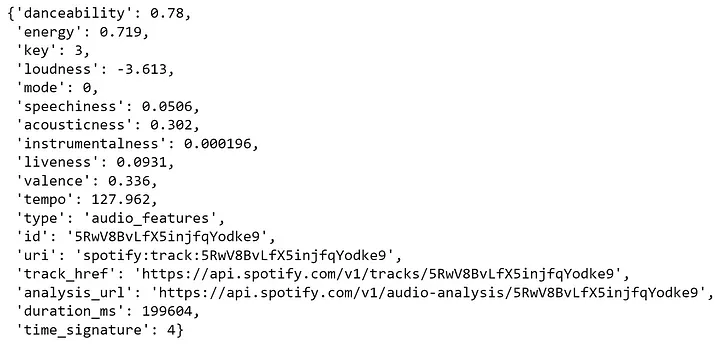
\includegraphics[width=1\linewidth]{images/spotify_data.png}
    \caption{Spotify API features [13].}
    \label{fig:enter-label}
\end{figure}

\subsection{Enrichment of Node Information using Spotify API}
To extend our analysis of song-song co-occurrence networks, we're able to utilise the Spotify API in order to extract semantic features like 'danceability' and 'energy'. These given examples are more abstract in their nature compared to more concrete features like 'tempo' or 'time{\_}signature, but they provide a rich foundation on which to analyze the relationship between target songs in a playlist. By using these attributes, we can 're-calibrate' and 'enrich' the network's centrality measures to see if we can find any correlations with the enriched information; it also allows us to go beyond our traditional network analysis by considering auxiliary and more holistic elements of the playlist network, potentially unravelling other attributes that may/may not have an influence over the songs that are present in more playlists. \\

\begin{figure}[h!]
    \centering
    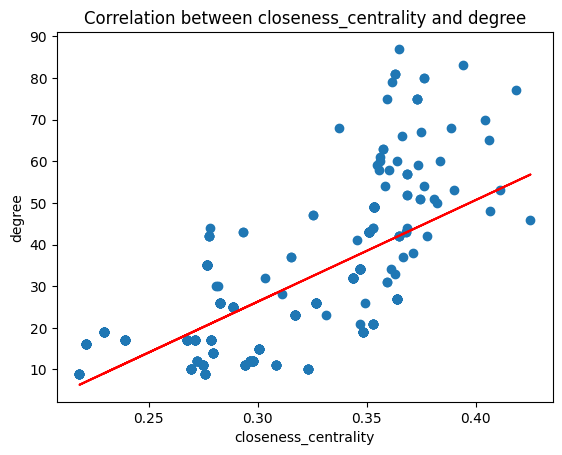
\includegraphics[width=1\linewidth]{images/ccvsd.png}
    \caption{Closeness Centrality vs. Node Degree}
    \label{fig:enter-label}
\end{figure}

% ------------------------------------------------------------ %

\section{Results and Discussion}

\begin{table*}[hbt!]
\centering
\caption{Network Statistics - Enriched Network Analysis}
\label{table:kysymys}
\begin{tabularx}{\textwidth}{@{} l *{10}{C} c @{}}

        \toprule
        Spotify API Metric & Small Network Average & Large Network Average & Change (+/-)\\
        \midrule
        Danceability & 0.6177 & 0.6348 & + \\
        Energy & 0.6520 & 0.6712 & + \\
        Valence &  0.5060 & 0.5106 & + \\
        Tempo & 118.8641 & 121.9188 & + \\
        Duration & 233888.1303 & 232287.9262 & - \\
        Popularity & 43.6405 & 45.1355 & + \\
        Acousticness & 0.2202 & 0.1765 & - \\
        Speechiness & 0.0834 & 0.0998 & + \\
        Liveness & 0.1845 & 0.1820 & - \\
        Instrumentalness & 0.0175 & 0.0135 & - \\
        Loudness & -6.7870 & -6.5535 & - \\
        \bottomrule
        
    \end{tabularx}

\end{table*}

\subsection{Large Network Analysis}

Transitioning to a more expansive scope, the network evolves to encompass 2,767 nodes with 229,384 edges. This scaled perspective broadens our comprehension of song inter-connectivity on a wider spectrum as well as highlighting particular details upon closer examination. At a glace we can observe that: \\

\begin{itemize}
    \item\textbf{Enhanced Connectivity and 'Hub' Tracks:} The maximum value for degree nodes jumped massively between the small and large datasets, going from (87) to (776) respectively. Thus illustrating that the larger dataset has far more connections within the network indicating that on average, that there is a higher presence of 'hub' songs than those in the smaller dataset. Notably, tracks such as "One Dance" emerge with heightened connectivity in the larger dataset. This observation amplifies the importance of cross-genre appeal and popularity as central attributes.
    
    \item\textbf{Diluted Genre Clustering:} A decrease in the clustering coefficient (0.582) suggests a diminishing emphasis on genre as the network expands, pivoting towards artist popularity and cross-playlist versatility as more prevalent factors due to greater musical diversification. \\
    
    \item\textbf{Elevated Closeness and Discoverability:} The diminished distance between nodes in the larger network underscores the rising prominence of attributes that facilitate discovery — namely, the versatility of songs and universal appeal elements like rhythm gaining much more importance, especially as a higher closeness centrality suggests that there is a tighter integration of songs that are closer to other nodes in the playlists. \\
    
    \item\textbf{Attribute Shift:} There is a subtle shift from the focus of intrinsic song characteristics such as genre and mood to extrinsic factors such as popularity and/or connectivity the larger the dataset expands; suggesting that the playlist generation algorithm may balance these characteristics for broader appeal, especially as there is a more diverse catalogue of songs found in playlists. \\

    \item\textbf{Eigenvector Discrepancy:} The minimum eigenvector value (8.1146) is shown with a much higher value compared to the small dataset (4.0842) and could suggest that the less influential nodes in the network are connected to influential network, meaning that it might still facilitate niche music discovery occasionally.
\end{itemize}

In summary, we can conclude that the larger and more diverse the network becomes, the more centrally oriented songs (i.e. mainstream songs) take center stage, and slowly overshadow niche genres unless they are heavily interlinked; especially as the positive correlation between closeness and degree highlights their accessibility in network distance to other nodes, with popular/mainstream songs tending to have a greater closeness. The reduced path lengths and eigenvector values of the network further suggest that it facilitates broad music discovery, leaning more towards popular and closely interlinked songs rather than more niche ones; further exasberated by the small-world effect illustrating that as the network expands, shorter paths are found between nodes and with some acting as 'hubs'. Additionally, it sheds a light on the challenges and strategies in balancing out how automatic playlist continuation might need to adjust for network size, suggesting the need for additional attributes in gauging recommendation algorithms in a fairer prospect.\\

\subsection{Enriched Network Analysis}
Using the Spotify API, The audio features were pulled in batches and appended to the node information in the datasets. The average metrics of each of these attributes were then calculated to see the potential effects they had on both the smaller and larger datasets and weather any distinctions could be made. What we discovered is that after enriching the information with various attributes such as 'danceability', 'energy', 'valence' etc. saw an increase from the small to large network averages, but also we saw some particular correlations between how these attributes may influence the network. For instance, when analysing the small graph, we found that there was a weak correlation between 'danceability' and closeness; however when the same analysis was conducted on the larger dataset, we found differing results. \\

\begin{figure}[h!]
    \centering
    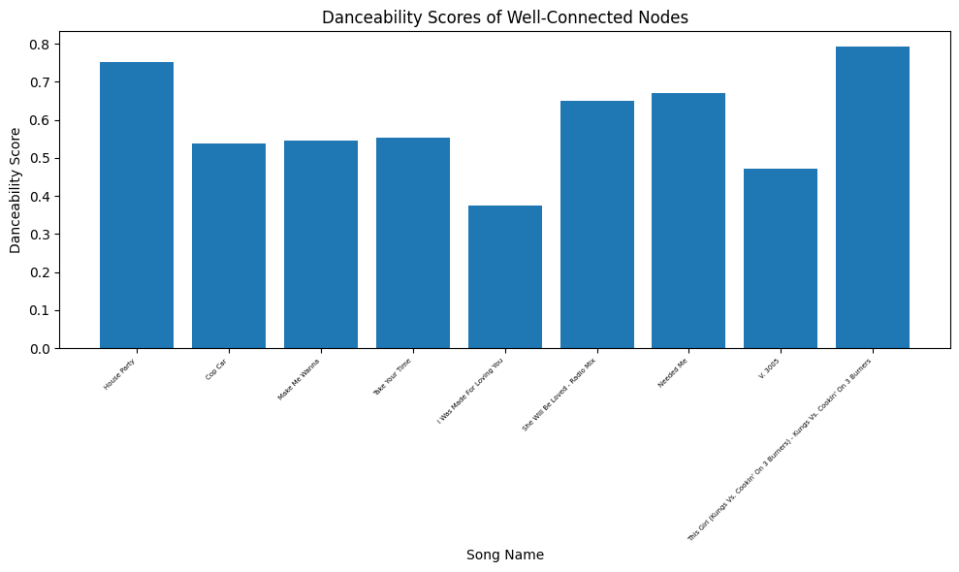
\includegraphics[width=1\linewidth]{images/wcn.png}
    \caption{Danceability scores of selected well connected nodes in the dataset (small)}
    \label{fig:enter-label}
\end{figure}

\begin{figure}[h!]
    \centering
    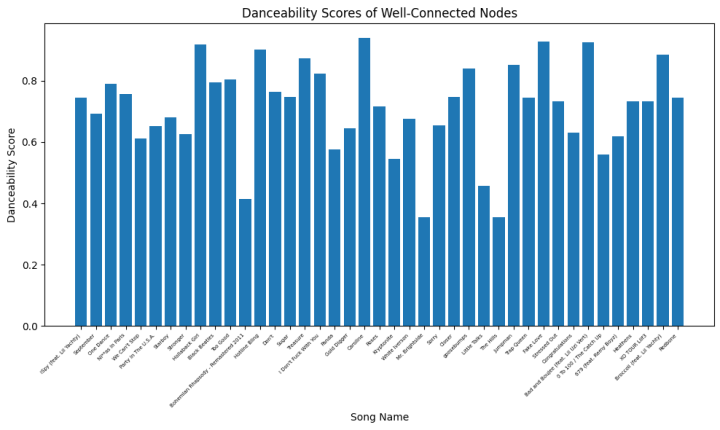
\includegraphics[width=1\linewidth]{images/songvsdanceability.png}
    \caption{Danceability scores of selected well connected nodes in the dataset (large)}
    \label{fig:enter-label}
\end{figure}

Our analysis reveals a significant consistency in the danceability attribute among well-connected songs in our co-occurrence networks on the large dataset. Specifically, the visualisation and quantification of danceability scores across these nodes show a strong clustering above the 0.6 mark, implying that highly danceable songs are more likely to be included in diverse playlists. \\

This trend not only emphasises the importance of danceability in the APC algorithms' decision-making processes, but it also reflects a wider user preference for rhythmically engaging tracks in playlist compositions. The absence of low-danceability outliers in well-connected positions suggests a possible algorithmic bias, favouring songs that meet specific rhythmic criteria and potentially contributing to a 'filter bubble' in which similar types of music are constantly recommended. We also found that there is a significant positive correlation between an artist's popularity and where they are in the playlist network, as evidenced by the correlation coefficient of 0.196 in the larger and smaller datasets. We can conclude from this empirical data that more well-known artists on Spotify typically hold key positions in the network, serving as hubs that are intricately linked to a vast array of other songs. \\

\begin{figure}[h!]
    \centering
    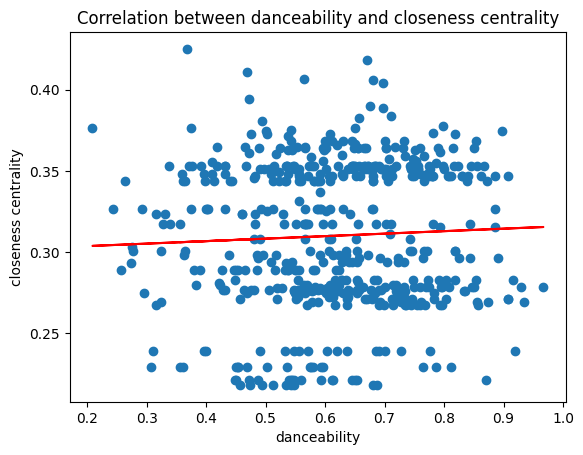
\includegraphics[width=1\linewidth]{images/1.png}
    \caption{Danceability vs. Closeness Centrality}
    \label{fig:enter-label}
\end{figure}

The observed slight positive correlation aligns with the theory that popular artists and by extension, their songs, serve as central nodes within the playlist network. These songs are positioned so that they are, on average, closer to the majority of other songs in the network. This centrality not only makes them accessible 'hubs' that connect many other tracks and genres, but it also reflects both consumers' and automatic playlist building algorithms' preference for well-known artists. These artists, due to their success, have a broader audience, meaning they are more likely to be present in a Spotify user's playlist, which in turn gives it a higher chance of being recommended by the algorithm. This is further exacerbated by the the platform's marketing and feature placements highlight these artists, increasing their visibility and likelihood of inclusion in several playlists. The scatter plots attached, while displaying variance, support this connection, with a clear trend line demonstrating that as artist popularity rises, so does their closeness and centrality in the network. This trend holds true across various data scales, reinforcing the idea that artist popularity is a significant driver of song interconnectedness within the network, potentially influencing music streaming service recommendations and shaping users' listening habits. 

\begin{figure}[h!]
    \centering
    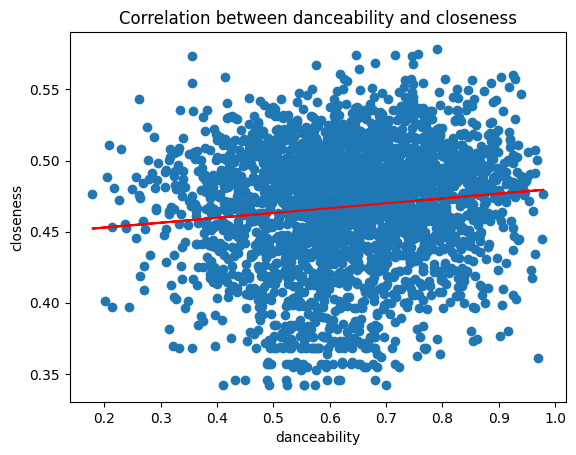
\includegraphics[width=1\linewidth]{images/2.png}
    \caption{Danceability vs. Closeness}
    \label{fig:enter-label}
\end{figure}

\begin{figure}[h!]
    \centering
    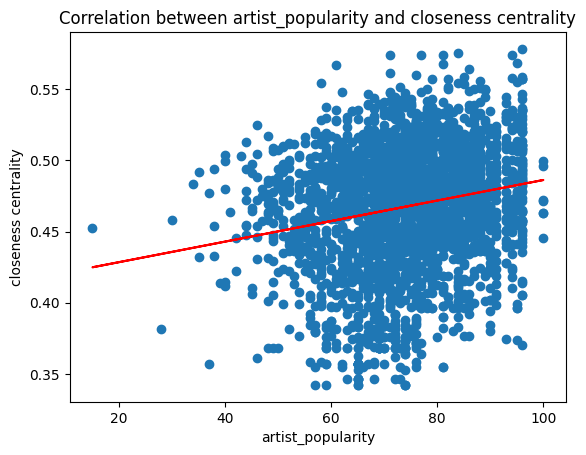
\includegraphics[width=1\linewidth]{images/3.png}
    \caption{Artist Popularity vs. Closeness Centrality}
    \label{fig:enter-label}
\end{figure}

\begin{figure}[h!]
    \centering
    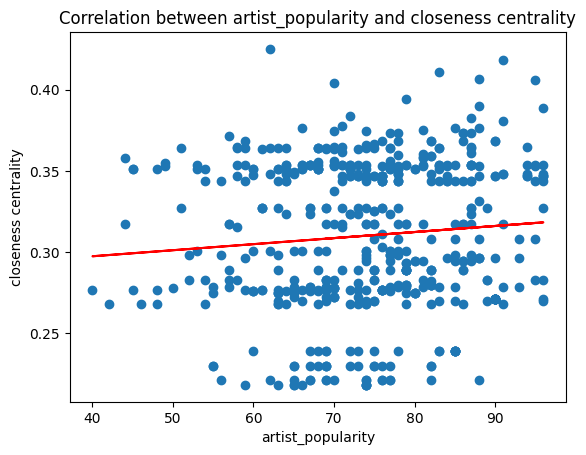
\includegraphics[width=1\linewidth]{images/4.png}
    \caption{Artist Popularity vs. Closeness Centrality}
    \label{fig:enter-label}
\end{figure}

When evaluating weather we can see if popular artists grouped together more often others, we can determine that since the recommendation algorithms tend to favour well known artists due to their broader appeal and promotion of higher user engagement, it may infer that popular artists frequently appearing together in playlists aims to maximise listener retention - shown between the artist popularity and the closeness centrality, highlighting a positive correlation; indicative that more popular songs may tend to appear clustered together in playlists due to their inherent broad appeal.
\\


% ------------------------------------------------------------ %

\section{Conclusions and Perspectives}

In conclusion, our study revolves around the analysis of network topology of music playlists, analysing the effects of centrality on network topology. Through studying co-occurrence networks derived from this playlist data, we found notable patterns and have provided various insights into the dominant attributes that influence playlist composition. \\

The comparison between small and large network characteristics revealed a shift towards mainstream songs and weaker genre clustering, and the prominence of centrality measures like degree and closeness underscores the importance of accessibility and popularity in playlist continuation algorithms. Moreover, when we extended the node information with the Spotify API, attributes such as danceability highlighted the influence of specific song characteristics on playlist inclusion. These findings reveal some of the simple underlying mechanisms of automatic playlist continuation and provide valuable insights for improving recommendation algorithms. By understanding the interplay between centrality, song attributes, and network topology, we can enhance the homogeneity and relevance of playlist recommendations for the users of these systems. \\

Future research could explore additional attributes and factors influencing playlist generation, as well as addressing potential biases and limitations in recommendation algorithms. By continuing to refine the understanding of playlist dynamics, we can better meet the evolving needs and preferences of music listeners in the digital age. \\

% ------------------------------------------------------------ %

\begin{thebibliography}{00}

% Yes
\bibitem{b1} Achahbar, A. and Lachgar, A. (2023) Uncovering the hidden structure of small-world networks [Preprint]. doi:10.21203/rs.3.rs-3249066/v1. \\

% Yes
\bibitem{b2} Bryan, N.J. and Wang, G. (2011) Musical Influence Network Analysis and rank of sample-based music., Proceedings of the 12th International Society for Music Information Retrieval Conference, ISMIR 2011. Available at: https://www.researchgate.net/publication/220723768{\_}Musical{\_}\\Influence{\_}Network{\_}Analysis{\_}and{\_}Rank{\_}of{\_}Sample-Based{\_}Music (Accessed: 05 April 2024). \\

% Yes
\bibitem{b3} Cano, P. et al. (2006) ‘Topology of Music Recommendation Networks’, Chaos: An Interdisciplinary Journal of Nonlinear Science, 16(1). doi:10.1063/1.2137622. \\

% Yes
\bibitem{b4} Chen, C.-W. et al. (2018) ‘Recsys Challenge 2018’, Proceedings of the 12th ACM Conference on Recommender Systems[Preprint]. doi:10.1145/3240323.3240342. \\

% Yes
\bibitem{b5} Deldjoo, Y., Schedl, M. and Knees, P. (2024) ‘Content-driven music recommendation: Evolution, state of the art, and challenges’, Computer Science Review, 51, p. 100618. doi:10.1016/j.cosrev.2024.100618. \\

% Yes
\bibitem{b6} Flexer, A. (2015) The impact of hubness on music recommendation, Machine Learning for Music Discovery Workshop at the 32nd International Conference on Machine Learning. Available at: https://ofai.at/papers/oefai-tr-2015-01.pdf (Accessed: 05 April 2024). \\

% Yes
\bibitem{b7} Goldrick, S. (2024) Smart Shuffle breathes new life into your Spotify playlists, Spotify. Available at: https://newsroom.spotify.com/2023-03-08/smart-shuffle-new-life-spotify-playlists/ (Accessed: 27 February 2024). \\

% Yes
\bibitem{b8} Hariri, N., Mobasher, B. and Burke, R. (2012) ‘Context-aware music recommendation based on latenttopic sequential patterns’, Proceedings of the sixth ACM conference on Recommender systems [Preprint]. doi:10.1145/2365952.2365979. \\

% Yes
\bibitem{b9} Jannach, D., Kamehkhosh, I. and Bonnin, G. (2016) ‘Biases in automated music playlist generation’, Proceedings of the 2016 Conference on User Modeling Adaptation and Personalization [Preprint]. doi:10.1145/2930238.2930283. \\

% Yes
\bibitem{b10} Liew, K. et al. (2022) Network analyses for Cross-Cultural Music popularity [Preprint]. doi:10.31234/osf.io/fp75z. \\

% Yes
\bibitem{b11} Lee, S.K., Cho, Y.H. and Kim, S.H. (2010) ‘Collaborative filtering with ordinal scale-based implicit ratings for mobile music recommendations’, Information Sciences, 180(11), pp. 2142–2155. doi:10.1016/j.ins.2010.02.004. \\

% Yes
\bibitem{b12} South, T., Roughan, M. and Mitchell, L. (2020) ‘Popularity and centrality in Spotify Networks: Critical transitions in Eigenvector Centrality’, Journal of Complex Networks, 8(6). doi:10.1093/comnet/cnaa050. \\

% Yes
\bibitem{b13} Watts, C. (2022) Extracting song data from the Spotify API using Python, Medium. Available at: https://towardsdatascience.com/extracting-song-data-from-the-spotify-api-using-python-b1e79388d50 (Accessed: 22 March 2024). \\

% Yes
\bibitem{b14} Yang, H. et al. (2018) ‘MMCF’, Proceedings of the ACM Recommender Systems Challenge 2018 [Preprint]. doi:10.1145/3267471.3267482. \\

% Yes
\bibitem{b15} Yürekli, A., Kaleli, C. and Bilge, A. (2021) ‘Alleviating the cold-start playlist continuation in music recommendation using latent semantic indexing’, International Journal of Multimedia Information Retrieval, 10(3), pp. 185–198. doi:10.1007/s13735-021-00214-5.

\end{thebibliography}

\vspace{12pt}

\section{Appendix}

\begin{figure}[htb!]
    \centering
    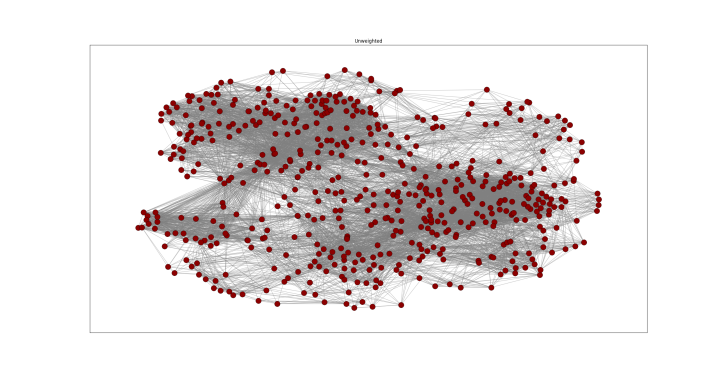
\includegraphics[width=1\linewidth]{images/unweighted.png}
    \caption{Unweighted Graph}
    \label{fig:enter-label}
\end{figure}

\begin{figure}[htb!]
    \centering
    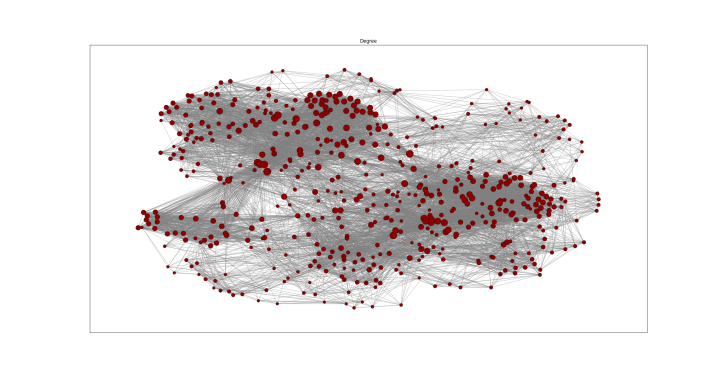
\includegraphics[width=1\linewidth]{images/degree.png}
    \caption{Degree}
    \label{fig:enter-label}
\end{figure}

\begin{figure}[htb!]
    \centering
    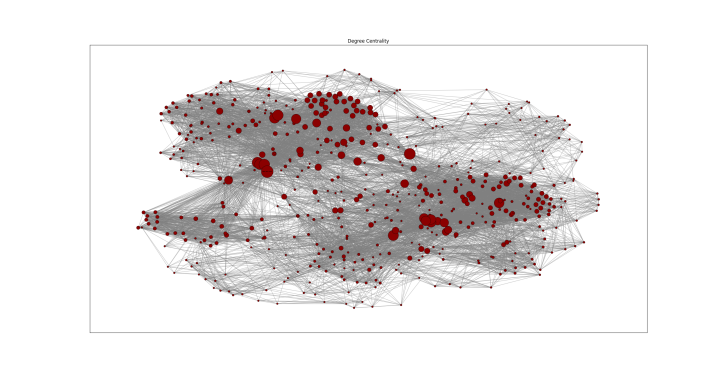
\includegraphics[width=1\linewidth]{images/degree_centrality.png}
    \caption{Degree Centrality}
    \label{fig:enter-label}
\end{figure}

\begin{figure}[htb!]
    \centering
    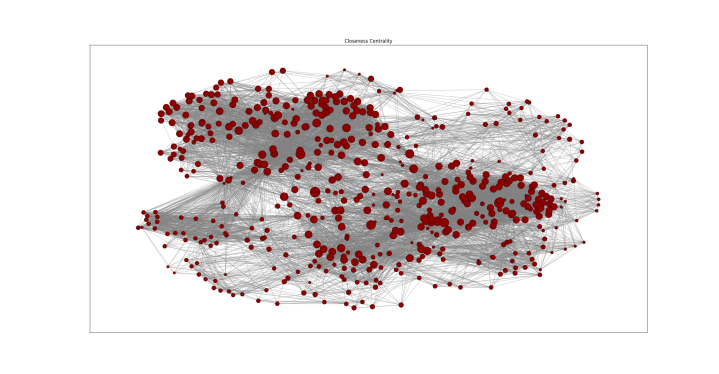
\includegraphics[width=1\linewidth]{images/closeness_centrality.png}
    \caption{Closeness Centrality}
    \label{fig:enter-label}
\end{figure}

\begin{figure*}
    \centering
    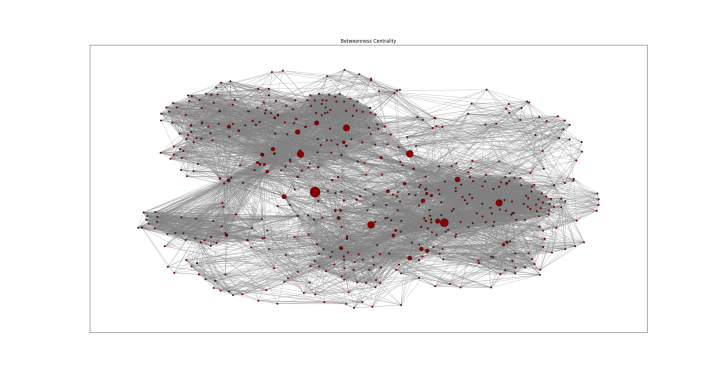
\includegraphics[width=1\linewidth]{images/betweenness_centrality.png}
    \caption{Betweenness Centrality}
    \label{fig:enter-label}
\end{figure*}

\begin{figure*}
    \centering
    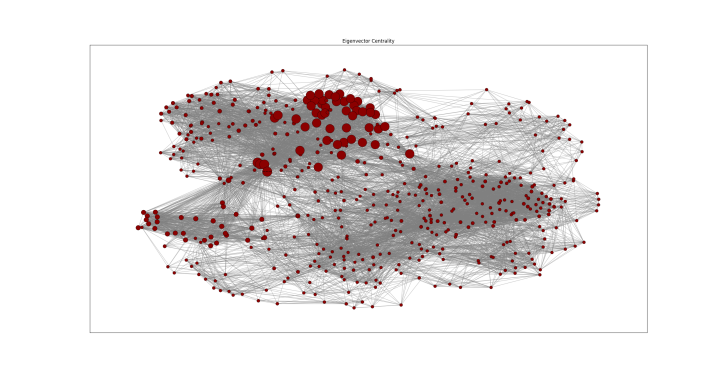
\includegraphics[width=1\linewidth]{images/eigenvector_centrality.png}
    \caption{Eigenvector Centrality}
    \label{fig:enter-label}
\end{figure*}

\end{document}
